%%%%%%%%%%%%%%%%%%%%%%%%%%%%%%%%%%%%%%%%%%%%%%%%%%%%%%%%%%%%%%%%%%%%%%%%%%%%%%%
%%%% Problem 3
%%%%%%%%%%%%%%%%%%%%%%%%%%%%%%%%%%%%%%%%%%%%%%%%%%%%%%%%%%%%%%%%%%%%%%%%%%%%%%%
\problem{3}
\subsubsection{Question}
% Keywords
	\index{thermodynamics!Mean free path of helium}

The cross-section for collisions between helium atoms is about \SI{e-16}{
\cm\squared}. Estimate the mean free path of helium atoms in helium gas at
atmospheric pressure and temperature.

\subsubsection{Answer}

Consider the path traced out by a helium atom as it travels a path length $L$,
colliding with other helium atoms along the way. Given that the cross section
of helium is $σ$, than we can estimate the volume that contains probable
interactions with our atom of interest as $\mathcal V = σL$. To get the number
of interactions, we make use of the fact that we're treating the gas as an
ideal gas. From the ideal gas law,
\begin{align*}
    PV &= NkT
\intertext{so that solving for the number density}
    n = \frac{N}{V} &= \frac{P}{k_B T}
\end{align*}
Combining the density with the volume, we get the number of other [point
particle] helium atoms that are contained within the given helium atom's
interaction volume. If we then assume that the atom interacts with all other
atoms within the volume, and that the collisions are spaced out equally in
time, we just have to normalize the value by the trajectory's path length to
get an estimate of the mean free path of helium in a helium gas:
\begin{align*}
    λ &= \frac{n\mathcal V}{L} = \frac{σP}{k_B T}
\end{align*}
Plugging in $σ = \SI{e-16}{\cm\squared}$, $P = \SI{1.013e5}{\Pa}$, $k_B =
\SI{1.38e-23}{\J\per\K}$, and $T = \SI{298}{\K}$, we get
\begin{empheq}[box=\fbox]{align}
    λ &= \SI{4.06}{\micro\m}
\end{empheq}


%%%%%%%%%%%%%%%%%%%%%%%%%%%%%%%%%%%%%%%%%%%%%%%%%%%%%%%%%%%%%%%%%%%%%%%%%%%%%%%
%%%% Problem 9
%%%%%%%%%%%%%%%%%%%%%%%%%%%%%%%%%%%%%%%%%%%%%%%%%%%%%%%%%%%%%%%%%%%%%%%%%%%%%%%
\problem{9}
\subsubsection{Question}
% Keywords
	\index{thermodynamics!Arbitrary engine efficiency}

An engine using \SI{1}{\mol} of an ideal diatomic gas performs the cycle $A
\rightarrow B \rightarrow C \rightarrow A$ as shown in the diagram below. $A
\rightarrow B$ is an adiabatic expansion, $B \rightarrow C$ occurs at
constant pressure, and $C \rightarrow A$ takes place at constant volume.
What is the efficiency of the cycle?

\begin{center}
    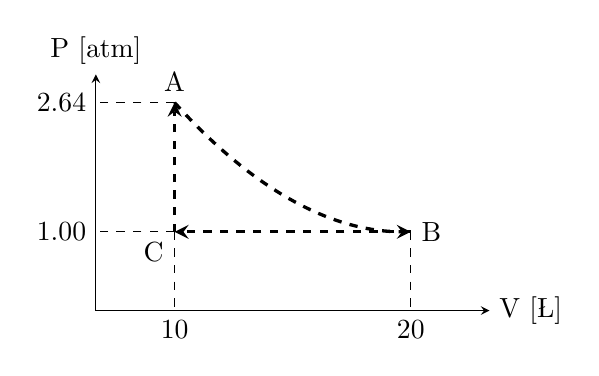
\begin{tikzpicture}[
	>=stealth
    ]
    % Draw the axes
	\draw [->] (0,0) -- (0,3) node [anchor=south] { P [\si{atm}] };
	\draw [->] (0,0) -- (5,0) node [anchor=west] {V [\si{\L}]};

	% Then draw the engine cycle
	\draw [very thick,dashed,->] (1,1)    -- (1, 2.64)
	    node [anchor=south] {A};
	\draw [very thick,dashed,->] (1,2.64) parabola[bend at end] (4,1)
	    node [anchor=west] {B};
	\draw [very thick,dashed,->] (4,1)    -- (1,1)
	    node [anchor=north east] {C};
	;

	% Then draw in the labels that give the absolute numbers
	\draw [dashed] (1,2.64) -- (0,2.64) node [anchor=east] {2.64};
	\draw [dashed] (1,1) -- (0,1) node [anchor=east] {1.00};
	\draw [dashed] (1,1) -- (1,0) node [anchor=north] {10};
	\draw [dashed] (4,1) -- (4,0) node [anchor=north] {20};
    \end{tikzpicture}
\end{center}

\subsubsection{Answer}

Since we want to find the efficiency of the cycle, we only care about the
heat exchanged during each stage of the cycle. Because the path $A
\rightarrow B$ is adiabatic, we immediately know that $Q = 0$. Then
proceeding to look at the stage $C \rightarrow A$, we know that the work
done during this cycle is identically zero since there is no area under the
curve. That means we are left simply with the equation
\begin{align*}
    dU = dQ
\end{align*}
Because this is an ideal [diatomic] classical gas, we combine the equations
\begin{align*}
    U &= \frac 52 nRT
\intertext{and}
    PV &= nRT
\end{align*}
to get that the difference in energy across the path is
\begin{align*}
    Q_{CA} &= U = \frac 52 nR(T_A - T_C) \\
    {}&= \frac 52 V₁ (P₂ - P₁)
\end{align*}

For the remaining stage $B \rightarrow C$, we use the full thermodynamic
identity:
\begin{align*}
    dU &= dQ - P\,dV
\end{align*}
The pressure $P₁$ is constant, so both integration of $dU$ and $dV$ are simply
the differences in each quantity. Again substituting for the temperature in
$U$ with the ideal gas law,
\begin{align*}
    \frac 52 nR(T_C - T_B) &= Q_{BC} - P₁(V₁ - V₂) \\
    \frac 52 P₁(V₁ - 2V₁) &= Q_{BC} + P(V₁ - 2V₁) \\
    Q_{BC} &= -\frac 72 P₁V₁
\end{align*}

We've accounted for all the heat flow in the system. $Q_{BC}$ is negative, so
this is the heat flow out of the system, while $Q_{CA}$ is positive and is the
heat flow into the system. By definition then, the efficiency $η$ of the system
is
\begin{align*}
    η &= 1 - \frac{Q_{out}}{Q_{in}} \\
    {}&= 1 - \frac{\frac 72 P₁ V₁}{\frac 52 V₁ (P₂ - P₁)} \\
    {}&= 1 - \frac 57 \frac{P₁}{P₂ - P₁}
\end{align*}
Plugging in the given values, we find the efficency to be
\begin{empheq}[box=\fbox]{align}
    η &= 0.146 = \SI{14.6}{\percent}
\end{empheq}

